\documentclass[a4paper,10pt]{article}
\usepackage[utf8]{inputenc}
\usepackage[spanish]{babel}
\usepackage[affil-it]{authblk}
\usepackage{enumerate}
\usepackage{graphicx}
\usepackage{hyperref}
\usepackage{amsmath}
\usepackage{amssymb}
\usepackage{cancel}
\usepackage[usenames, dvipsnames]{color}
\usepackage{tikz}
\usepackage{multimedia}
\usepackage{subcaption} %Multiple images
\usepackage{multicol} % Multiple columns
\usepackage{float}
\usepackage{cleveref}
\usepackage[margin=1.4in]{geometry}
\usepackage[labelfont=bf]{caption}
\usepackage[titletoc,toc,title]{appendix}
\usepackage{enumitem}
\usetikzlibrary{calc}
\numberwithin{equation}{section}

%Appendices in spanish
\renewcommand{\appendixname}{Ap\'endices}
\renewcommand{\appendixtocname}{Ap\'endices}
\renewcommand{\appendixpagename}{Ap\'endices}

%Zero delimiter
\newcommand{\zerodel}{.\kern-\nulldelimiterspace}

%Columns separation
\setlength{\columnsep}{1cm}

%Indentation
\setlength{\parindent}{0ex}

%Multiple References

\crefrangelabelformat{equation}{(#3#1#4--#5\crefstripprefix{#1}{#2}#6)}

\usepackage{xparse}
\ExplSyntaxOn
\NewDocumentCommand{\mref}{m}{\quinn_mref:n {#1}}
\seq_new:N \l_quinn_mref_seq
\cs_new:Npn \quinn_mref:n #1
 {
  \seq_set_split:Nnn \l_quinn_mref_seq { , } { #1 }
  \seq_pop_right:NN \l_quinn_mref_seq \l_tmpa_tl
  ( % print the left parenthesis
  \seq_map_inline:Nn \l_quinn_mref_seq
    { \ref{##1},\nobreakspace } % print the first references
  \exp_args:NV \ref \l_tmpa_tl 
  ) 
 }
\ExplSyntaxOff


%Boxes

\newcommand*{\boxcolor}{blue}
\makeatletter
\renewcommand{\boxed}[1]{\textcolor{\boxcolor}{%
\tikz[baseline={([yshift=-1ex]current bounding box.center)}] \node [rectangle, minimum width=1ex,rounded corners,draw] {\normalcolor\m@th$\displaystyle#1$};}}
 \makeatother

%Constantes
\newcommand{\euler}{\mathrm{e}}
\newcommand{\im}{i}

%Lemas, teoremas, definiciones y pruebas
\newcommand{\definicion}{\textbf{Definición: }}
\newcommand{\lema}{\textbf{Lema: }}
\newcommand{\teorema}{\textbf{Teorema: }}
\newcommand{\prueba}{\textbf{Prueba: }}
\newcommand{\proposicion}{\textbf{Proposición: }}


%opening
\title{Mecánica Clásica Tarea \# 8}
\author{Favio Vázquez\thanks{Correo: favio.vazquezp@gmail.com}}\affil{Instituto de Ciencias Nucleares. Universidad Nacional Autónoma de México.}
\date{}

\begin{document}

\makeatletter
\def\@maketitle{%
  \newpage
  \null
  \vskip 2em%
  \begin{center}%
  \let \footnote \thanks
    {\Large\bfseries \@title \par}%
    \vskip 1.5em%
    {\normalsize
      \lineskip .5em%
      \begin{tabular}[t]{c}%
        \@author
      \end{tabular}\par}%
    \vskip 1em%
    {\normalsize \@date}%
  \end{center}%
  \par
  \vskip 1.5em}
\makeatother

\maketitle

\section{Problema 1}

Construya un atlas para el toro de dos dimensiones.

\vspace{.3cm}

\underline{Solución:} \vspace{.3cm}

\section{Problema 2}

Demuestre que la estructura de espacio vectorial que se dio al conjunto de clases de 
tangencia de curvas que pasan por un punto de una variedad diferencial, es independiente 
de las cartas utilizadas y de las curvas representativas escogidas en cada clase.

\vspace{.3cm}

\underline{Solución:} \vspace{.3cm}

\section{Problema 3}

Demuestre que la definición de diferencial en un punto de un mapeo entre dos variedades 
diferenciales es buena y que proporciona un mapeo lineal que se reduce a la noción 
común de diferencial cuando las dos variedades son espacios de tipo $\mathbb{R}^n$.

\vspace{.3cm}

\underline{Solución:} \vspace{.3cm}

\section{Problema 4}

Demuestre que el conjunto que denotamos por 

$$
\left( \frac{\partial}{\partial q^1},\dots, \frac{\partial}{\partial q^n}\right)
$$

es una base para el espacio tangente de una variedad en el punto con coordenadas 
locales $(q^1,\dots,q^n)$.

\vspace{.3cm}

\underline{Solución:} \vspace{.3cm}

\section{Problema 5}

Identifique la variedad de configuración correspondiente a las rotaciones de un cuerpo 
rígido. Demuestre que los ángulos de Euler son un sistema de coordenadas para esa 
variedad.

\vspace{.3cm}

\underline{Solución:} \vspace{.3cm}

\definicion Un cuerpo rígido es un sistema de $N$ partículas puntuales, constreñidas 
por relaciones holonómicas expresadas por el hecho de que la distancia entre los 
puntos es constante:

\begin{equation}
 |\mathbf{r}_i - \mathbf{r}_j| = \text{constante},
\end{equation}

para todo $i,j = 1,\dots,N$.

\vspace{.3cm}

El movimiento más general para un cuerpo rígido es una traslación más una rotación 
sobre un punto $P$, pero para la solución de este problema solo consideraremos las 
rotaciones.

\vspace{.3cm}

Sea un cuerpo rígido fijado en un punto $P$. Consideremos una rotación sobre el punto 
$P$. Para describir esto, especificaremos las posiciones en un marco de referencia 
estático $\{{\tilde{\mathbf{e}}_a\}}$ introduciendo un marco de referencia en movimiento $\{{\mathbf{e}_a}\}$
en el cuerpo de manera que $\{\mathbf{e}_a\}$ se mueve con él. Debajo se encuentra una 
ilustración de estas consideraciones,

\begin{figure}[H]
 \center 
 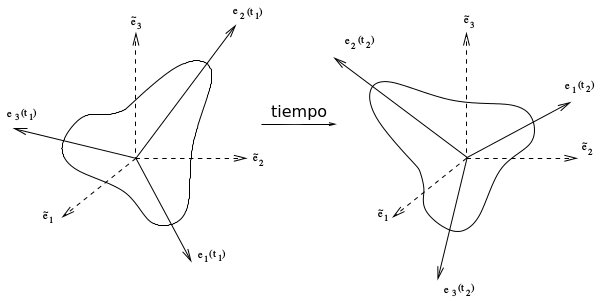
\includegraphics[scale=0.6]{problema5fig1}
 \caption{El marco de referencia estático y el marco de referencia en movimiento.}
\end{figure}

Debido a que ambos ejes son ortogonales, tenemos que 

\begin{equation}
 \tilde{\mathbf{e}}_a \cdot \tilde{\mathbf{e}}_b = \delta_{ab}, \quad \mathbf{e}_a(t) \cdot \mathbf{e}_b(t) = \delta_{ab}.
\end{equation}

\proposicion Para todo $t$, existe una matriz ortogonal única $R(t)$ con componentes 
$R_{ab}(t)$ tal que $\mathbf{e}_a(t) = R_{ab}(t)\tilde{\mathbf{e}}_b$.

\vspace{.3cm}

\prueba $\mathbf{e}_a \cdot \mathbf{e}_b = \delta_{ab} \Rightarrow R_{ac}R_{bd} 
(\tilde{\mathbf{e}}_c\cdot\tilde{\mathbf{e}}_d) = \delta_{ab} \Rightarrow R_{ac}R_{bc} = 
\delta_{ab}$ o, en otras palabras, $(R^TR)_{ab} = \delta_{ab}$ lo cual establece que 
$R$ es ortogonal. La unicidad de $R$ proviene de la construcción $R_{ab} = \mathbf{e}_a \cdot 
\tilde{\mathbf{e}}_b$.

\vspace{.3cm}

Entonces mientras el cuerpo rígido rota, esta rotación es descrita por una matriz 
$3\times 3$ ortogonal y dependiente del tiempo $R(t)$. Debido a la propiedad de 
las matrices $R$, $R_{ac}R_{bc} = \delta_{ab}$, y al hecho de que esta matriz es 
real, puede probarse sin dificultad que éstas tienen determinantes $\pm 1$. Debido 
a que todas las rotaciones físicas pueden ser alcanzadas continuamente de la 
la transformación idéntica (ángulo cero de rotación), y debido a que el determinante 
de esta es $+1$, entonces todas las matrices de rotación deben tener determinante $+1$, 
a este tipo de matrices se les llama matrices especiales. Entonces, cada familia uniparamétrica $R(t)$ describe un posible movimiento para 
el cuerpo, y llegamos a la siguiente conclusión:

\begin{center}
 $M$ = Variedad de configuración para  las rotaciones del cuerpo rígido = Espacio de las matrices 
 ortogonales especiales $\equiv$ \textbf{SO(3)}.
\end{center}

\vspace{.3cm}

Una matriz $3\times 3$ tiene $9$ componentes pero la condición de ortogonalidad $R^TR=1$
impone $6$ relaciones, por lo tanto la variedad de configuración es tridimensional, y 
por lo tanto necesitamos $3$ coordenadas generalizadas para parametrizar y describir 
completamente a $M$. Como probaremos en el siguiente teorema, estas coordenadas son 
los conocidos ángulos de Euler.

\teorema Una rotación arbitraria puede ser expresada como el producto de $3$ rotaciones 
sucesivas sobre (en general) $3$ ejes diferentes.

\vspace{.3cm}

\prueba Sean $\{{\tilde{\mathbf{e}}_a\}}$ los ejes del sistema estático y 
$\{{\mathbf{e}_a\}}$ los ejes anclados al cuerpo en rotación. Queremos encontrar 
la rotación $R$ tal que $\mathbf{e}_a = R_{ab}{\tilde{\mathbf{e}}_b}$. Podemos 
lograr esto en tres pasos

\begin{equation}
 \{{\tilde{\mathbf{e}}_a\}} \xrightarrow{R_3(\phi)} 
 \{{\mathbf{e}'_a\}} \xrightarrow{R_1(\theta)} 
 \{{\mathbf{e}''_a\}} \xrightarrow{R_3(\psi)} \{{\mathbf{e}_a\}}
\end{equation}

\textbf{Paso 1}: Rotación por un ángulo $\phi$ sobre el eje $\tilde{\mathbf{e}}_3$. 
Entonces $\mathbf{e}'_a = R_3(\phi)_{ab}\tilde{\mathbf{e}}_b$ con 

\begin{equation}
 R_3(\phi) = \begin{pmatrix}
              \cos{\phi} & \sen{\phi} & 0 \\
	      -\sen{\phi} & \cos{\phi} & 0 \\
	      0 & 0 & 1
	     \end{pmatrix}.
\end{equation}

\begin{figure}[H]
  \center 
  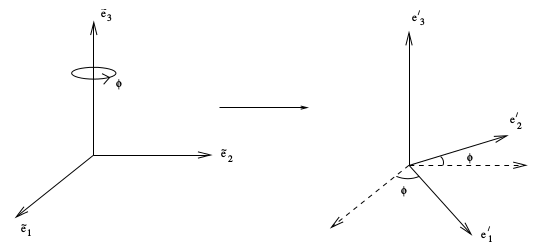
\includegraphics[scale=0.6]{problema5fig2}
  \caption{Paso 1: Rotación sobre $\tilde{\mathbf{e}}_e$ del marco de referencia 
  estático.}
\end{figure}

\textbf{Paso 2}: Rotación por un ángulo $\theta$ sobre el nuevo eje $\mathbf{e}'_1$. 
Este eje $\mathbf{e}'_1$ es conocido como la ``línea de nodos''. Escribimos entonces 
$\mathbf{e}''_a = R_1(\theta)\mathbf{e}'_b$ con 

\begin{equation}
 R_3(\theta) = \begin{pmatrix}
              1 & 0 & 0 \\
	      0 & \cos{\theta} & \sen{\theta} \\
	      0 & -\sen{\theta} & \cos{\theta}
	     \end{pmatrix}.
\end{equation}

\begin{figure}[H]
  \center 
  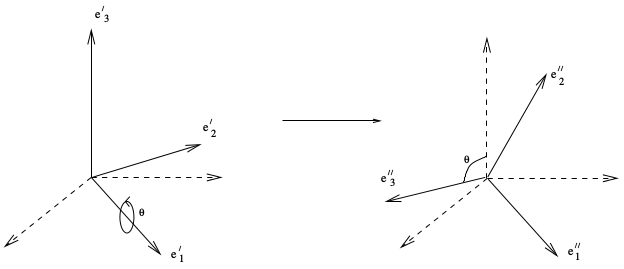
\includegraphics[scale=0.6]{problema5fig3}
  \caption{Paso 2: Rotación sobre el nuevo eje $\mathbf{e}'_1$.}
\end{figure}

\textbf{Paso 3}: Rotación por un ángulo $\psi$ sobre el nuevo eje $\mathbf{e}''_3$ 
entonces $\mathbf{e}_a = R_3(\psi)_{ab}\mathbf{e}''_b$ con 

\begin{equation}
 R_3(\psi) = \begin{pmatrix}
              \cos{\psi} & \sen{\psi} & 0 \\
	      -\sen{\psi} & \cos{\psi} & 0 \\
	      0 & 0 & 1
	     \end{pmatrix}.
\end{equation}

Poniendo todo esto junto tenemos que 

\begin{equation}
 R_{ab} (\phi,\theta,\psi) = [R_3(\phi)R_1(\theta)R_3(\psi)]_{ab}
\end{equation}

Los ángulos $\phi,\theta,\psi$ son los ángulos de Euler. Los cuales hemos demostrado 
entonces que forman un sistema de coordenadas para la variedad de configuración 
para las rotaciones de un cuerpo rígido, ya que podemos escribir la matriz $R(\phi,\theta,\psi)$
como 

\begin{equation*}
 R  = \begin{pmatrix}
              \cos{\psi}\cos{\phi} - \cos{\theta}\sen{\phi}\sen{\psi} & 
              \sen{\phi}\cos{\psi} + \cos{\theta}\sen{\psi}\cos{\phi} & 
              \sen{\theta}\sen{\psi} \\
	      -\cos{\psi}\sen{\psi} - \cos{\theta}\cos{\psi}\sen{\phi} & 
	      -\sen{\psi}\sen{\phi} + \cos{\theta}\cos{\psi}\cos{\phi} & 
	      \sen{\theta}\cos{\psi} \\
	      \sen{\theta}\sen{\phi} & -\sen{\theta}\cos{\phi} & \cos{\theta}
	     \end{pmatrix},
\end{equation*}

y esta cumple con las propiedades deseadas para probar el teorema que hemos propuesto 
y para formar un sistema de coordenadas locales para \textbf{SO(3)}. Cabe destacar 
que al utilizar estos ángulos para un problema concreto, debemos recordar que este 
sistema de coordenadas es similar a las coordenadas geográficas sobre la esfera: excluyen 
los polos y son multivaluadas en un meridiano.

\end{document}
